\documentclass{article}
\usepackage{fullpage}
\usepackage{graphicx}
\usepackage{url}

\title{Limitations}

\author{Gordon Reid - 1002536r}

\begin{document}

\maketitle

\section{MPI LES}

\subsection{Halo Boundaries}

Compare Figure~\ref{fig:standardLESGrid} and Figure~\ref{fig:mpiLESGrid}. Both
grids have the same depth however, for the sake of brevity, this is not shown in
the diagram.

The standard LES grid is two kinds of boundary: periodic boundary and open
boundary. The periodic boundary are simple memory copies between one side of the
grid to another. The open boundary is merely a copy to the neighbouring row of
the grid.

The MPI LES grid is split into a certain number of processors per row and per
column as shown by the inner, smaller, sections. The grid has the same periodic
and open boundaries however, in the case of the period boundaries, the exchange
is actually an MPI message between two processes, one pair per row. In addition
to these boundaries, the MPI grid also has halo exchanges between the internal
sections. Up to four exchanges (up, down, left and right) may be required
because, to calculate a value at position (x, y), a process needs to know its
neighbouring values which, without the halo exchange, would be out of range for
the outer edges of a process' grid section.

The boundary code is found in four files: bondFG.f95, bondv1.f95, boundp.f95 and
boundsm.f95. Halo exchanges and period boundary side exchanges need to be added
to these files. MPI exchanges come at a non-zero cost so performance concerns
immediately come to mind. For bondFG.f95, bondv1.f95 and boundsm.f95 this should
not be an issue given that they are called once per timestep however boundp.f95
is called four times per timestep. At the cost of correctness, boundp.f95 may
need to be ignored in terms of MPI exchanges in order to achieve suitable
performance numbers.

An additional problem occurs when considering corner values. The four halo
exchanges do not include the corners, these come from the grid that's up-left,
up-right, down-left, down-right from the process. This means that, per array
section, the halo exchange would need to be eight messages instead of four. This
would cause an unacceptable performance hit thus the corner values are estimated
based on the three neighbouring values known to the process at the cost of
absolute correctness.

\subsection{Effect of Corner Estimation in Halo Boundaries}

As shown by a Github Issues comment
\footnote{\url{https://github.com/gordon1992/LES-WRF-MPI/issues/15#issuecomment-65896162}}
the corner estimation code makes a difference to output. Taking the original LES
code and executing it on a 37x37x90 example with and without corner estimation
code resulted in differing timesteps where non-convergence occurred. This does
not suggest a place where corner estimation makes a difference but shows that it
has some effect on the data. Only a single place needs to exist where estimated
values are used to calculate another value for the difference to occur. Once
this occurs the effect of the estimation will `infect' the rest of the array,
radiating out from the estimated corner. This was found in netCDF output for
pressure in the MPI version where there was a slightly different value for
pressure compared to the original non-estimated code radiating out from corners
of the array.

Places where corner estimated values are used:

\begin{itemize}
    \item les.f95\\
    ! --calculation of sgs eddy viscosity coeficient\\
    - dudyx1 = ... diu2(i-1,j+1,k) ... - Top Right\\
    - dvdxx1 = ... diu4(i+1,j-1,k) ... - Bottom Left\\
    These are then used to calculate values for sm\\
    sm is then used to calculate values for eddyviscosity values\\
    eddyviscosity values are then used to calculate values for f, g, and h.
\end{itemize}

\begin{figure}
    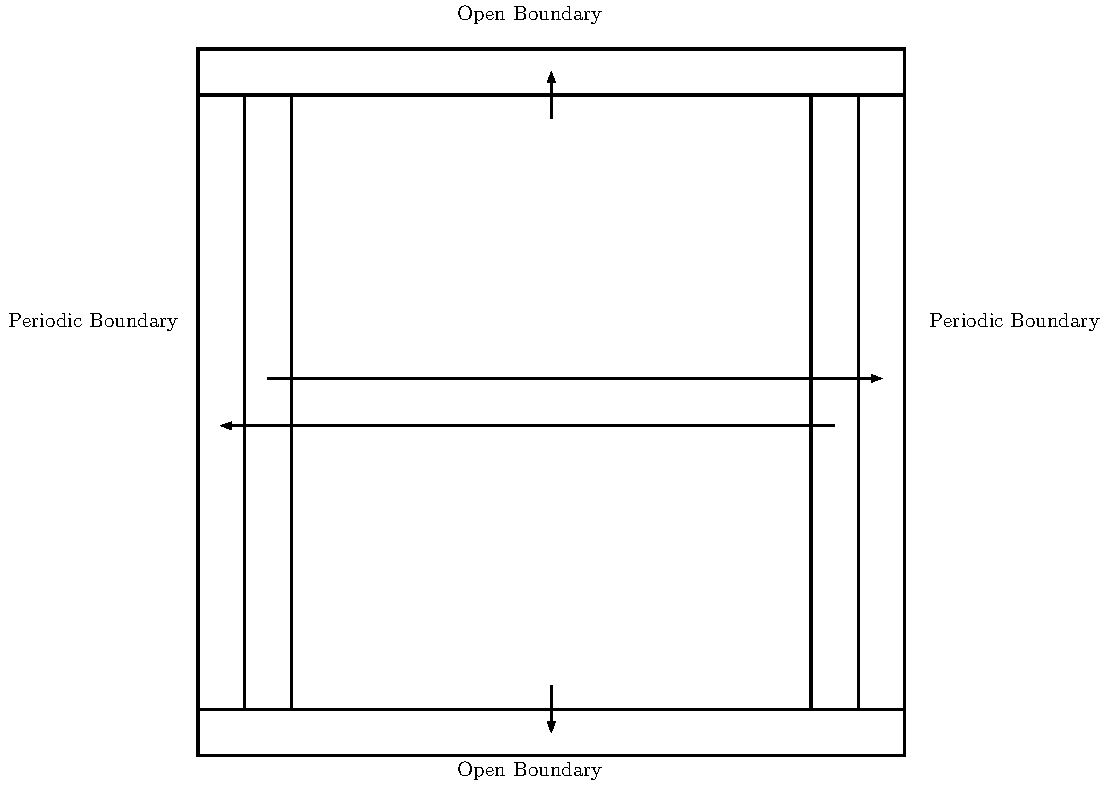
\includegraphics[width=\linewidth]{Diagrams/standardLESGrid.pdf}
    \caption{Standard LES Grid}
    \label{fig:standardLESGrid}
\end{figure}

\begin{figure}
    \includegraphics[width=\linewidth]{Diagrams/mpiLESGrid.pdf}
    \caption{MPI LES Grid}
    \label{fig:mpiLESGrid}
\end{figure}

\end{document}
